\clearpage
\section*{\currfilename}

\pgfdeclarelayer{background}
\pgfdeclarelayer{foreground}
\pgfsetlayers{background,main,foreground}

% Define a few styles and constants
\tikzstyle{sensor}=[draw, fill=blue!20, text width=5em, text centered, minimum height=2.5em]
\tikzstyle{ann} = [above, text width=5em]
\tikzstyle{naveqs} = [sensor, text width=6em, fill=red!20, minimum height=12em, rounded corners]

\def\blockdist{4.5}
\def\edgedist{2.5}

\begin{tikzpicture}
  \node (block3) [squareblock, label=below:{\shortstack[c]{\bf Nonlinear Equations\\ \bf of Motion}}, minimum width=6cm, inner sep=0mm] {\centering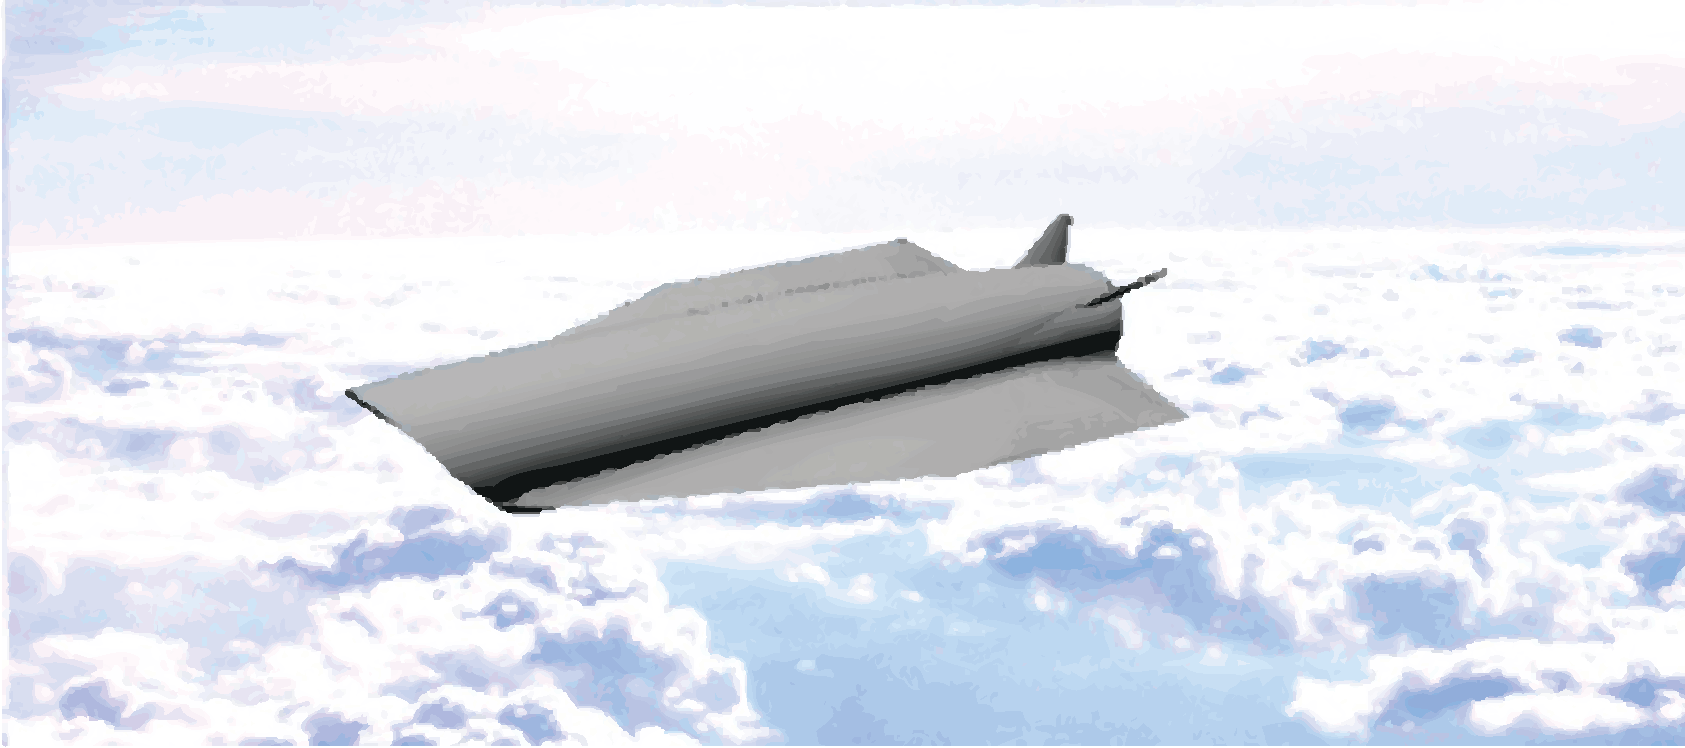
\includegraphics[width=6cm]{../fig/ghvclouds.pdf}};
  \node (naveq) [naveqs] {Navigation equations};
  \path (naveq.145)+(-\blockdist,0) node (block1) [squareblock, minimum width=2.5cm] {Baseline};
  \path (naveq.-145)+(-\blockdist,0) node (block2) [squareblock, minimum width=2.5cm] {\shortstack{Adaptive \\ Augmentation}};
  \node (sum1) [whitesum, right of=block3, node distance=4.5cm] {};
  \node (input1) [input, above of=sum1, node distance=1.5cm] {};
  \node (output1) [input, right of=sum1, node distance=1.5cm] {};
  \path [draw, ->] (block1) -- (block3.west |- block1) ;
  \path [draw, ->] (block2) -- (block3.west |- block2);
  %\path [draw, ->] (block3) -- node[pos=0.7]{$-$} (sum1);
  %\path [draw, ->] (input1) -- node[pos=0.2]{target} node[pos=0.7]{$+$} (sum1);
  %\path [draw, ->] (sum1) -- node[pos=0.7]{error} (output1);
  \draw[->](block3) -- node[pos=0.7, anchor=north]{$-$} (sum1);
  \draw[->](input1) -- node[pos=0.2, anchor=west]{target} node[pos=0.7, anchor=west]{$+$} (sum1);
  \draw[->](sum1) -- node[pos=0.7, anchor=south]{error} (output1);
\end{tikzpicture}
